\chapter{Introduction}\label{chap:intro}
\newtheorem{theorem}{Theorem}[section]
\newtheorem{proposition}{Proposition}[section]
\newtheorem{lemma}{Lemma}[section]
\newtheorem{corollary}{Corollary}[section]

\section{Weierstrass Equation}
The Weierstrass form of an elliptic curve $E$ over a field $K$ is given by the equation
\begin{equation}
y^2 = x^3 + Ax + B 
\end{equation}
with $A, B \in K$ and $4A^3 + 27B^2 \neq 0$.
\section{Group Law} \label{Group_Law}
Let $E$ be an elliptic curve defined by $y^2 = x^3 + Ax + B$, and let $P_1 = (x_1, y_1)$ and $P_2 = (x_2, y_2)$ be points on $E$ with $P_1, P_2 \neq \infty$. Define $P_1 + P_2 = P_3 = (x_3, y_3)$ as follows:
\begin{enumerate}
    \item If $x_1 \neq x_2$, then
    \begin{align*}
        x_3 &= m^2 - x_1 - x_2, \\
        y_3 &= m(x_1 - x_3) - y_1,
    \end{align*}
    where $m = (y_2 - y_1)/(x_2 - x_1)$.
    \item If $x_1 = x_2$ but $y_1 \neq y_2$, then $P_1 + P_2 = \infty$.
    \item If $P_1 = P_2$ and $y_1 \neq 0$, then
    \begin{align*}
        x_3 &= m^2 - 2x_1, \\
        y_3 &= m(x_1 - x_3) - y_1.
    \end{align*}
    where $m = (3x_1^2 + A)/(2y_1)$
    \item If $P_1 = P_2$ and $y_1 = 0$, then $P_1 + P_2 = \infty$.
\end{enumerate}
We know that $P_1, P_2 \in E$ and $(P_1 + P_2) \in E$. Therefore $E(K)$ is closed under the addition of above points.
\begin{definition}
We define the point at infinity as the additive identity element of the group law on the curve.
\begin{equation}
    P + \infty = P \quad \forall P \in E
\end{equation}
\end{definition}

\begin{theorem}
The addition of points on an elliptic curve $E$ satisfies the following properties:
\begin{enumerate}
    \item (Commutativity) $P_1 + P_2 = P_2 + P_1$ for all $P_1, P_2$ on $E$.
    \item (Existence of identity) $P + \infty = P$ for all points $P$ on $E$.
    \item (Existence of inverses) Given $P$ on $E$, there exists $P'$ on $E$ with $P + P' = \infty$. This point $P'$ will usually be denoted $-P$.
    \item (Associativity) $(P_1 + P_2) + P_3 = P_1 + (P_2 + P_3)$ for all $P_1, P_2, P_3$ on $E$.
\end{enumerate}
The points on $E$ form an additive Abelian group with $\infty$ as the identity element.
\end{theorem}
\begin{proof}
The line through P1 to P2, is the same as the line through P2 to P1. Therefore the point $(P_1 + P_2)$ will be the same as the point $(P_2+P_1)$. Thus it is commutative. The identity property of $\infty$ holds by definition. Let $P'$ be the reflection of the point $P$ with respect to x axis. Then $P + P' = \infty$. Thus inverse exists for a given point $P$ in $E$. The proof of associativity can be found here $^{\cite{Washington:book:2008}}$.
\end{proof}

%% Below code taken from https://gist.github.com/tscholl2/b5d7a64fe9d283ee2b2bfe46588237a7
\begin{center}
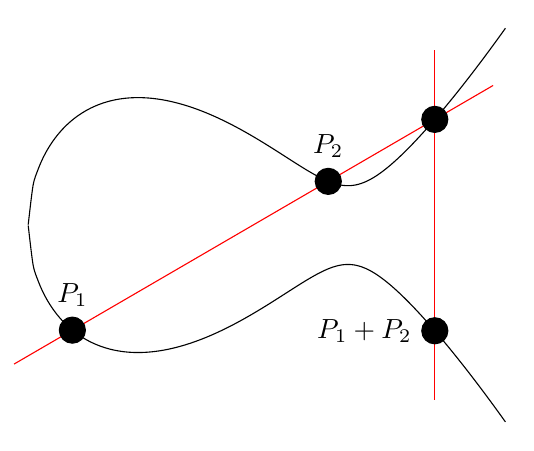
\begin{tikzpicture}[yscale=0.5]
%TODO: up sample size
\draw[domain=-4.060646:2,samples=100,smooth,variable=\x,black] plot ({\x},{sqrt(\x^3 + 4*(\x)^2 + 1)});
\draw[domain=-4.060646:2,samples=100,smooth,variable=\x,black] plot ({\x},{-sqrt(\x^3 + 4*(\x)^2 + 1)});
\node (P_1) at (-3.5, -2.66926956300783) {};
\node (P_2) at (-0.25, 1.1102430216445) {};
\node (R) at (1.10295826812394, 2.68474117626385) {};
\node (P_1+P_2) at (1.10295826812394, -2.68474117626385) {};
\draw[color=red,shorten >=-1cm,shorten <=-1cm] (P_1) -- (R);
\draw[color=red,shorten >=-1cm,shorten <=-1cm] (R) -- (P_1+P_2);
\node[circle,draw=black,fill=black,label=above:{$P_1$}] at (P_1) {};
\node[circle,draw=black,fill=black,label=above:{$P_2$}] at (P_2) {};
\node[circle,draw=black,fill=black] at (R) {};
\node[circle,draw=black,fill=black,label=left:{$P_1+P_2$}] at (P_1+P_2) {};
 \end{tikzpicture}
\end{center}

\subsection{Integer times a Point}
If we need to calculate the point $kP$, performing $k$ additions of $P$ can be computationally costly. To solve this problem, we can use the algorithm of successive doubling to compute $kP$ for a point $P$ on the Elliptic curve $E$ defined over the field $K$.

%% Algorithm taken from tetxbook
\begin{algorithm}
\caption{Successive doubling to find $kP$}\label{kp_algo}
\begin{algorithmic}[1]
\Procedure{multiply}{$k,P$}\Comment{to find the point $kP$}
\State $a\gets k$
\State $B\gets \infty$
\State $C\gets P$
\If{$a\bmod 2=0$}
\State $a\gets a/2$
\State $B\gets B$
\State $C\gets C+C$
\Else
\State $a\gets a-1$
\State $B\gets B + C$
\State $C\gets C$
\EndIf 
\If{$a\neq 0$}
\State Go to Step 5
\EndIf 
\State \textbf{return} $B$\Comment{$kP = B$}
\EndProcedure
\end{algorithmic}
\end{algorithm}

\section{Endomorphism}
\begin{definition}
    let $\alpha$ be a homomorphism. $\alpha : E(\Bar{K}) \rightarrow E(\Bar{K})$ that is given by rational functions $R_1(x,y), R_2(x,y)$ with coefficients in $\Bar{K}$, such that
    \begin{align*}
        \alpha(x,y) = (R_1(x,y), R_2(x,y)) \quad \forall (x,y) \in E(\Bar{K})
    \end{align*}
    Then $\alpha$ is an endomorphism of $E$.
\end{definition}

\subsection{Degree of $\alpha$}
Below is a standard form for the rational functions describing an endomorphism $\alpha$ of an elliptic curve given in Weierstrass form.
\begin{align*}
    \alpha(x,y) = (r_1(x), r_2(x)y) 
\end{align*}
where $r_1(x)$ and $r_2(x)$ are rational functions and
\begin{align*}
    r_1(x) = \frac{p(x)}{q(x)}
\end{align*}
where the polynomials $P(x)$ and $q(x)$ do not have a common factor.

\begin{definition}
    We define degree of $\alpha$ to be
    \begin{equation*}
         \operatorname{deg}(\alpha) = Max\{ \operatorname{deg}(p(x)),  \operatorname{deg}(q(x))\}
    \end{equation*}
    When $\alpha$ is non-trivial. If $\alpha = 0$, then $ \operatorname{deg}(\alpha) = 0$.
\end{definition}

\subsection{Separable Endomorphism}
\begin{definition}
    $\alpha \neq 0$ is said to be a separable endomorphism if the derivative $r_1'(x)$ is not identically zero
\end{definition}

\subsection{Frobenius Map}
\begin{definition}
    Suppose $E$ is an elliptic curve defined over the finite field $\mathbb{F}_q$. Let
    \begin{equation}
        \phi_q(x, y) = (x^q, y^q)
    \end{equation}
    Then $\phi_q$ is the Frobenius map 
\end{definition}

\begin{lemma}
    Let $E$ be defined over $\mathbb{F}_q$. Then $\phi_q$ is an endomorphism of $E$ of degree $q$, and $\phi_q$ is not separable.
\end{lemma}
\begin{proof}
   Let $(x_1, y_1), (x_2, y_2) \in E(\mathbb{F}_q)$ with $x_1 \neq x_2$\\
   Let $(x_3, y_3) \in  E(\mathbb{F}_q) $ such that $(x_3, y_3) = (x_1, y_1) + (x_2 + y_2)$
   \[\phi_q(x_3, y_3) = (x_3^q, y_3^q)\]
   Using the definition in \ref{Group_Law}
   \[m^q = \left(\frac{y_2-y_1}{x_2-x_1}\right)^q\]
   all the coefficients in the expansion except for $y_2^q$, $y_1^q$, $x_2^q$, $x_1^q$ will be a multiple of $q$, therefore
   \[ m^q = \frac{y_2^q - y_1^q}{x_2^q - x_1^q}\]
   let $m' = m^q$, then
   \[x_3^q = (m^2 - x_1 - x_2)^q\]
   all the coefficients in the expansion except for $m^{2q}$, $x_1^q$, $x_2^q$ will be a multiple of $q$, therefore
   \[x_3^q = m'^2 - x_1^q - x_2^q\]
   similarly we get,
   \[y_3^q = m'(x_1^q - x_3^q) - y_1^q\]
   Thus,
   \[\phi_q(x_3, y_3) = \phi_q(x_1, y_1) + \phi_q(x_2, y_2)\]
   We can check for the other cases similarly.\\
   Therefore $\phi_q$ is a homomorphism given by rational functions and thus is an endomorphism of $E$. \\
  $qx^{q-1}$ in $\mathbb{F}_q$ is zero as $q$ is zero in $\mathbb{F}_q$. Therefore derivative of $x^q$ is identically zero. Hence $\phi_q$ is not separable.
\end{proof}


\phantomsection

\begin{proposition}
    Let $\alpha \neq 0$ be a separable endomorphism of an elliptic curve $E$.Then 
    \begin{align*}
      \operatorname{deg}(\alpha) = \# \operatorname{Ker}(\alpha), 
    \end{align*}
    where $\operatorname{Ker}(\alpha)$ is the kernel of the homomorphism $\alpha: E(K) \rightarrow E(K)$.
    If $\alpha \neq 0$ is not separable, then 
    \begin{align*}
        \operatorname{deg}(\alpha) > \# \operatorname{Ker}(\alpha)
    \end{align*}
\end{proposition}

\begin{proof}
    Refer to $\cite{Washington:book:2008}$ for the proof. 
\end{proof}

\section{Torsion Points}
Let $E$ be an elliptic curve defined over field $K$. Let $n$ be a positive integer then, 
\begin{align*}
   E[n] = \{P \in E(K) \mid nP = \infty\}
\end{align*}

\begin{theorem}
    Let $E$ be an elliptic curve over a field $K$ and let $n$ be a positive integer. If the characteristic of $K$ does not divide $n$, or is 0, then
\[ E[n] \cong \mathbb{Z}_n \oplus \mathbb{Z}_n \]
If the characteristic of $K$ is $p > 0$ and $p \mid n$, write $n = p^r n'$ with $p \nmid n'$. Then
\[ E[n] \cong \mathbb{Z}_{n'} \oplus \mathbb{Z}_n \quad or \quad \mathbb{Z}_n \oplus \mathbb{Z}_{n'} \]
\end{theorem}
 
\section{Elliptic Curves over Finite Fields}
Let $\mathbb{F}$ be a finite field. Let $E$ be an elliptic curve defined over $\mathbb{F}$. Since there are only finitely many possible pairs $(x,y) \quad s.t \quad x,y \in \mathbb{F}$, The group $E(\mathbb{F})$ is finite.
\begin{theorem}
    Let $E$ be an elliptic curve over a field $\mathbb{F}_q$. Then
\[ E(\mathbb{F}_q) \cong \mathbb{Z}_n \quad or \quad \mathbb{Z}_{n_1} \oplus \mathbb{Z}_{n_2} \]
For some integer $n \geq 1$, or for some integers $n_1,n_2 \geq 1$ with $n_1$ dividing $n_2$.
\end{theorem}

\begin{theorem}{[Hasse's Theorem]}
    Let $E$ be an elliptic curve over a field $\mathbb{F}_q$. Then the order of $E(\mathbb{F}_q)$  satisfies
    \[\left|q + 1 - \#E(\mathbb{F}_q)\right| \leq 2\sqrt{q}\]
\end{theorem}

\begin{proof}
    Refer to $\cite{Washington:book:2008}$ for the above proofs.
\end{proof}
\newpage
\subsection{Order of Points}
Let P be a point on the Elliptic curve $E$ over a field $\mathbb{F}_q$. \\
Let $\#E(\mathbb{F}_q) = N$, By Lagrange's theorem, we know that $NP = \infty$. \\
By using Hasse's theorem we can try all values in the range $(q+1-2\sqrt{q}, q+1+2\sqrt{q})$ and check which one satisfies. This takes around $4\sqrt{q}$ steps.\\
We can speed up to around $4q^{1/4}$ steps using the baby step, giant step method to find the order of point P.

\begin{algorithm}
\caption{Baby Step, Giant Step method to find order of point $P$}\label{BSGS_ORDER}
\begin{algorithmic}[1]
\Procedure{bsgsorder}{$P$}\Comment{Compute order of point P}
\State $Q\gets (q+1)P$
\State Choose an integer $m$ such that, $m \geq q^{\frac{1}{4}}$
\For{$j=0$ to $m$}
\State compute and store $jP$
\EndFor
\For{$k=-m$ to $m$}
\State compute $Q + k(2mP)$
\If{$Q + k(2mP) = \pm jp$}
\State break \Comment{$(q + 1 + 2mk\mp j)P = \infty$}
\EndIf
\EndFor
\State $M\gets (q + 1 + 2mk) \mp j$
\State Factor $M$, $p_1,...p_r$ are the distinct prime factors of $M$
\For{$i=1$ to $r$}
\State $val \gets (\frac{M}{p_i})P$
\If{$val = \infty$}
\State $M\gets (\frac{M}{p_i})$
\State go to step 14
\Else
\State break
\EndIf
\EndFor
\State \textbf{return} $M$\Comment{order of $P$ is $M$}
\EndProcedure
\end{algorithmic}
\end{algorithm}
\newpage
\subsubsection{Correctness of Baby Step, Giant Step Method to find order of P}
\begin{lemma} \label{1.5.1}
    Let $a$ be an integer with $|a| \leq 2m^2$. There exists integers $a_0$ and $a_1$ with $-m \leq a_0, a_1 \leq m$ such that
    \[a = a_0 + 2ma_1\]
\end{lemma}
\begin{proof}
    let $a_0 \equiv a \pmod{2m}$, with $-m \leq a_0 \leq m$. let $a_1 = \frac{(a-a_0)}{2m}$
    \[|a - a_0| \leq |a| + |a_0| \leq 2m^2 + m\]
    \[\implies |a_1| \leq \frac{2m^2 + m}{2m} < m+1 \]
    \[-m \leq a_1 \leq m \]
\end{proof}
\noindent According to Hasse's theorem: 
\[q+1-2\sqrt{q} \leq N \leq q+1+2\sqrt{q}\]
\[\implies N = q + 1 - a \quad with \quad |a| \leq 2\sqrt{q}\]
At step-7 of the algorithm let $k = -a_1$ ($k$ lies in between $-m$ to $m$), Then using \ref{1.5.1}, there exists an integer $a_0 \in [-m, m]$
\[Q - a_1(2mP) = (q+1-2ma_1)P = (q+1-a+a_0)P = NP + a_0P = a_0P\]
Therefore at step-8 of the algorithm for $j = |a_0|$ there is a match.

\begin{lemma}
    Let $G$ be an additive group (with identity element $0$) and let $g \in G$. Suppose $Mg=0$ for some positive integer $M$. Let $p_1,...,p_r$ be the distinct primes dividing M. if $(M/p_i)g \neq 0$ for all $i$, then $M$ is the order of $g$.
\end{lemma}
\begin{proof}
    let $k$ be the order of $g$. The $k|M$ as $Mg=0$. Let $k \neq M$.\\
    Let $p_i$ be a prime divisor of $M/k$.
    \begin{align*}
        \implies p_ik|M 
        \implies k|(M/P_i) 
        \implies (M/P_i)g = 0
    \end{align*}
    Which is a contradiction, as we assumed $(M/p_i)g \neq 0$ for all $i$.\\
    Therefore $k=M$
\end{proof}
\noindent Therefore Steps 15 to 21 find the order of P.